\documentclass{article}

\usepackage{amsmath}
\usepackage{graphicx}
\usepackage{xcolor}
\usepackage[export]{adjustbox}
\RequirePackage[margin=1in]{geometry}

\newcommand\todo[1]{\textcolor{red}{TODO: #1}}

\newcommand\animation[1]{\textcolor{blue}{ANIMATION: #1}}

\begin{document}
	
\title{Hillshade Video Script}
\author{Nathan Stouffer}
\date{}
\maketitle

\section{Intro}

\subsection{Motivation}

When you look at the map shown below, I bet much of the terrain's shape is evident to you.
I'd guess that know this spot to be pretty flat and this other area to be relatively steep.
Possibly you can pick out a gully right here and a ridgeline over there.
Or maybe you've noticed that this face is pretty rugged while this slope is relatively smooth.

Regardless of what individual features you've noticed, I'm certain you have some notion of what this terrain looks like even though all you can see is a greyscale image.

This map is intentionally set up so that your brain can intuit the shape of the terrain.
Computers do much of this work today, but cartographers have been using this technique for hundreds of years.
And many other applications utilize similar strategies to convey geometric information.

\subsection{Topic}

The topic I'd like to discuss today is a lighting technique called hillshade.
We're going to see why it's an effective method of illumination and walk through the math that powers it.

\begin{center}
	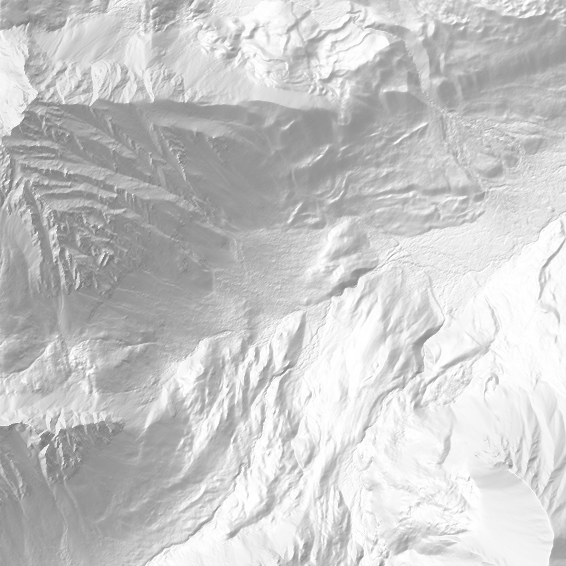
\includegraphics[width=0.5\textwidth,frame]{assets/hillshade-example.png}
\end{center}

\section{DirectionalLighting}

\subsection{EffectGraph}

The particular topic we'll be discussing is hillshade, but it's worth mentioning that hillshade is a very specific example of something called a directional light.
Directional lights are used all over computer graphics and are themselves just one option for how you might want to light a scene.
What I find so intriguing about directional lights is that they give you a lot of bang for your buck.
You get pretty realistic lighting for the expended level of effort.

\animation{Fade in a graph similar to the below image.}

\begin{center}
	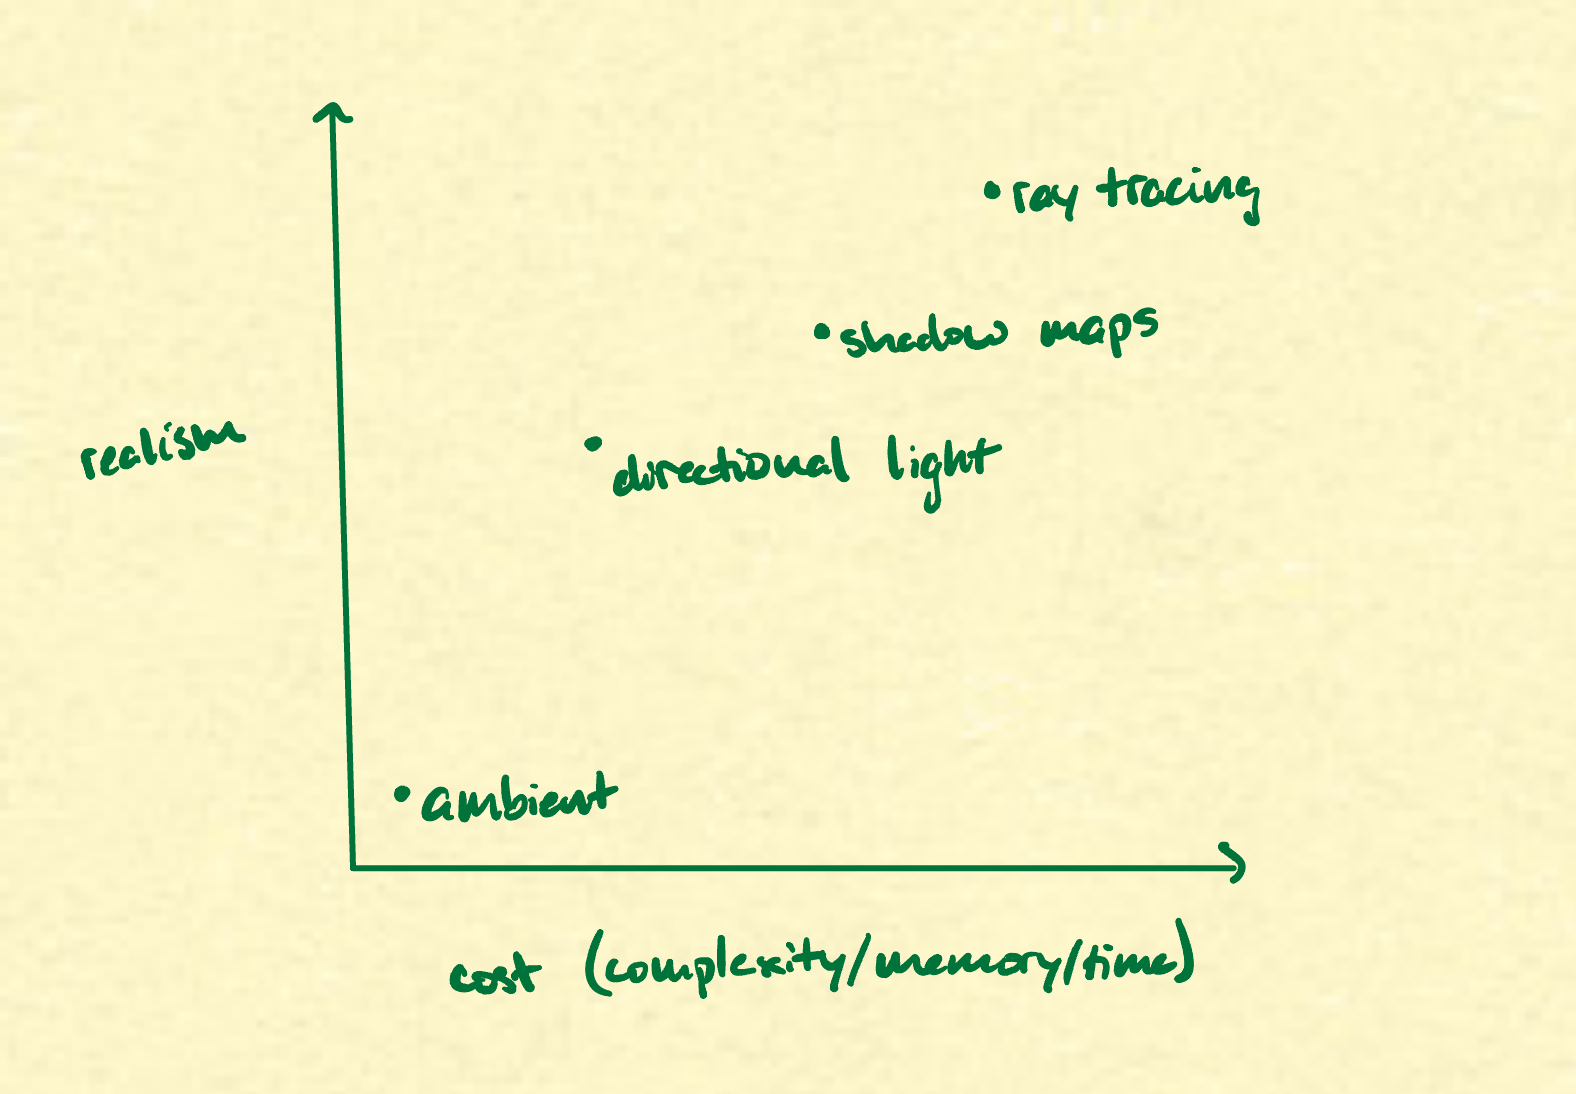
\includegraphics[width=0.65\textwidth,frame]{assets/realism.jpg}
\end{center}

If you were to represent different lighting techniques as points in the plane where the y-axis represents some notion of how realistic a scene looks and the x-axis represents some notion of cost (maybe in terms of complexity/memory/computation time).
Then on that plane, directional lights would exist at an extremely effective sweet spot -- they don't cost that much but they provide a healthy amount of realism.

\subsection{Assumptions}

Let's get into the details of what a directional light is.
A directional light is a pseudo-realistic model of how light behaves.
If we have a light source, an object, and an obstruction, then real light behaves something like this.
Directional lights make a few simplifying assumptions:

\begin{enumerate}

\item First, they ignore obstructions -- meaning we won't compute true shadows.
This is the piece of directional lights that I find to be the most interesting: even with this simplification, directional lights give enough hints of realism to trick your brain into thinking objects are 3-dimensional.

\animation{Demonstrate a simple example of shadows in 2D}.
	
\item Second, directional lights assume the light source to be extremely far away.
This means that every point in the scene has light coming from the same direction $l$.
It's also the reason for the ``direction" in the term directional lighting.

To make the math a little cleaner, we're actually going to reverse that direction.
This makes $l$ the vector that points directly \textit{towards} the light source.

\end{enumerate}

\subsection{DesiredBehavior}

The direction that the terrain faces is encoded in something called a surface normal.
If we zoom in very close to the terrain, then it can be reasonably approximated as a small plane.
The outward pointing vector that is orthogonal to that plane is called the surface normal.

\animation{Show a rotating plane with a surface normal that is lit according to hillshade.}

The effect we are looking for should behave like this:
If the terrain generally points in the same direction as the light, we want to use a pretty bright shade.
If the light direction kind of glances off the terrain, we want to shade with a tone of grey.
And if the terrain generally faces away from the light direction, we want to use a dark shade.

\section{Derivation}

\subsection{ShadowArea}

At this point, we've covered what the effect should do, but how can we accomplish it?
What are the nuts and bolts that turn this loose discussion into something we can compute?

We can start by more precisely describing how the light strength should vary.
Let's represent a small area of the terrain as a rotated square.
We'll establish that when the vector pointing towards the light source $l$ and the surface normal $n$ point in the exact same direction, we want to light at full strength -- which is to say that the terrain should be colored white.
Next, we know that we want to decrease the strength of the light as the angle between $n$ and $l$ increases.
To root our model in reality, we can vary the intensity of the shading based on how much light is blocked by the rotated square - ie the area of its shadow.

I won't prove this for you, but it so happens that (with a directional light) the signed area of a rotated square's shadow is the square's area $A$ times $\cos \theta$ where $\theta$ is the angle between $l$ and $n$.
The sign of the result encodes whether or not the square faces the light source (positive means facing towards the light and negative means facing away).
If an un-rotated square gets the full light strength of $1$, then this fact implies that a rotated square gets strength $S = 1 * \cos \theta = \cos \theta$.

\subsection{TransformCosine}

You might notice that $\cos \theta$ can be negative.
What are we to do with a negative light strength?
Well, it depends on the application.
Some directional light models ignore negative light strengths by clamping to 0.
With hillshade, our goal is to effectively illuminate a map so that the reader can see terrain features.
When we ignore negative light strengths, we remove shading on all terrain that faces away from the light source.
Instead, it is more effective to remap the range of cosine to the interval $[0, 1]$.
This can be done by first adding 1 and then dividing by 2.
 
\animation{Transform the range of cosine via $\dfrac{1}{2}(1 + \cos \theta)$}

\begin{center}
	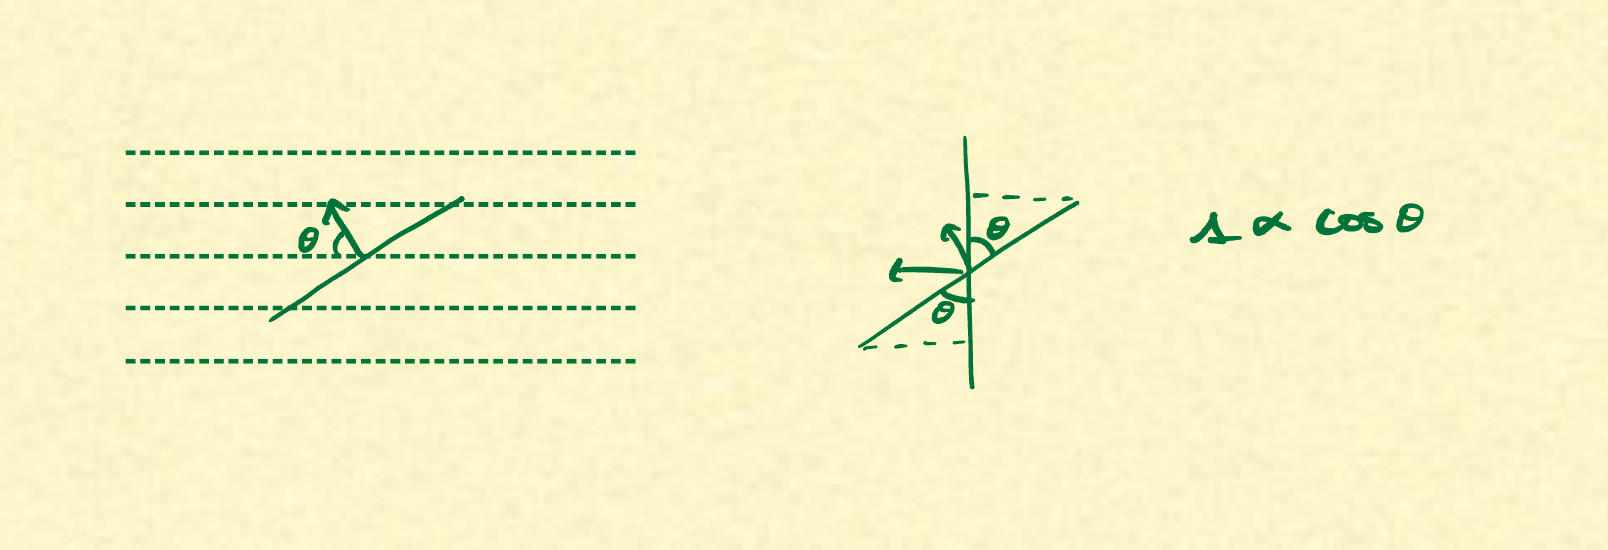
\includegraphics[width=0.75\textwidth,frame]{assets/cosine.jpg}
\end{center}

\subsection{WhatIsLink}

We have figured out that computing the shading strength depends on $\cos \theta$ -- where $\theta$ is the angle between our two vectors.
But that doesn't really help us much because we don't know what $\theta$ is -- all we know are the vectors $l$ and $n$.
At the end of the day, those are just lists of numbers.
What is the link between these two vectors and cosine?

The trick is to bring a triangle into the mix.
We are going to draw the third leg of our triangle here and use the Law of Cosines.

\begin{center}
	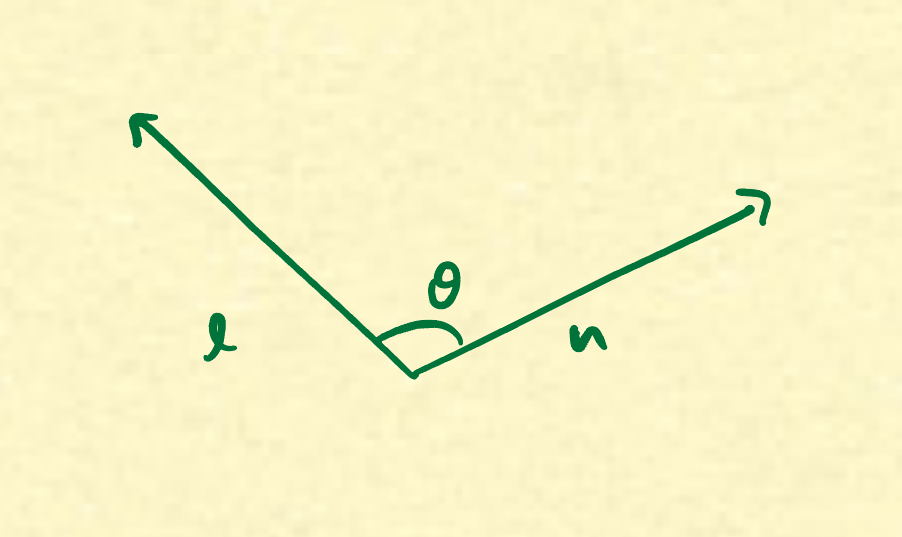
\includegraphics[width=0.3\textwidth,frame]{assets/ln.jpg}
	\hspace{0.2\textwidth}
	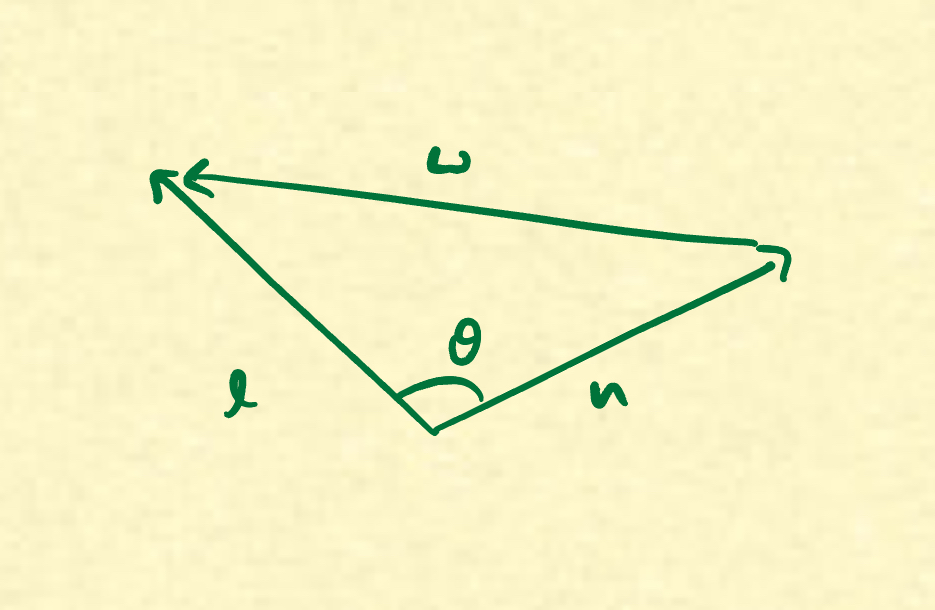
\includegraphics[width=0.2735\textwidth,frame]{assets/lnw.jpg}
\end{center}

\subsection{LawOfCosines}

The full Law of Cosines says that for any triangle with sides/angle labeled like so, we have the following equality: $c^2 = a^2 + b^2 - 2ab \cos C$.
In our case, $a = |l|$, $b = |n|$, and the angle $C = \theta$.
The third side of our triangle is the difference between $l$ and $n$ so its length is magnitude of that difference.

\begin{align*}
|l-n|^2 = |l|^2 + |n|^2 - 2 |l| |n| \cos \theta & \quad \text{substitute from generalized LoC} \\
|l-n|^2 = 2 - 2 \cos \theta & \quad \text{didn't discuss this earlier, but } |l| = |n| = 1 \\
1 - \dfrac{1}{2}|l-n|^2 = \cos \theta & \quad \text{simplifying}
\end{align*}

I didn't mention this earlier, but by convention, $l$ and $n$ are chosen to be unit vectors -- meaning their magnitude is 1.
If we use that fact and then simplify, we can compute $\cos \theta$ from values that we already know: the vectors $l$ and $n$.

If you are familiar with the dot product, you know that this can be further simplified into some really compact notation.
But in the interest of accessibility, I'm going to leave it here because we have what we need.

\section{Hillshading}

\subsection{FinalProduct}

From our shadow area discussion, we know the strength of our light is $\dfrac{1}{2}(1 + \cos \theta)$ and we just figured out how to compute $\cos \theta$ in terms of the two things we know: the vectors $l$ and $n$.
Computing that value for each pixel is all it takes to produce the beautiful images shown here.
It never ceases to amaze me how such simple a computation can produce stunning and realistic results.

\animation{Show a few examples.}

\subsection{Endnotes}

\subsubsection{Variations (about 25s)}

I'd like to close the video by making a few comments.

First, hillshade isn't just one thing.
It's actually a term for a family of effects that can be applied to a map.
There are a lot of variations out there.
Some add ambient light, exaggerate the terrain, use multiple light sources, or play around with colors.
You now have the mathematical framework that sits behind all of them.

\todo{Possibly mention Eduard Imhof.}

\subsubsection{Pseudoscopic Illusion (about 30s)}

Second, most people have an easier time recognizing terrain features when the light is placed in the top left of an image.
Because many maps place north at the top edge of the screen, hillshade is typically lit from the northwest.

However, this can sometimes backfire when that same map is oriented with \textit{south} at the top edge of the screen.
When that occurs, your brain \textit{might} interpret everything backwards (ie valleys as ridges and ridges as valleys).
This is called a pseudoscopic illusion.

\animation{Show a south-up map light from the northwest and then fade in the same map (still south up) with a southeast (top left) light}.

\subsubsection{Simplicity (about 30s)}

For my final comment, I'd like revisit the simplicity of this effect -- I just can't get over it!
The math works out to be pretty simple and yet the results are unreasonably effective.
But what's even crazier is the fact that all the maps you've seen in this video are 2-dimensional -- and I don't just mean that the screen you're viewing is 2D.
The actual model I am rendering is a square in the plane.

\animation{Pitch the camera}

Despite that, hillshade vividly evokes the 3-dimensional nature of terrain.

\animation{3D flythrough?}

\end{document}